\documentclass[11pt]{report}

% Language and font stuff
\usepackage[utf8]{inputenc}
\usepackage[english]{babel}
\usepackage{csquotes}
\usepackage[T1]{fontenc}
\usepackage[final]{microtype}

\usepackage[bookmarks]{hyperref}

% Formatting options
\usepackage[margin=1in]{geometry}
\setlength{\parindent}{0pt}
\setlength{\parskip}{3pt}

% Math commands
\usepackage{amsmath,amssymb,amsthm}

\theoremstyle{plain}
\newtheorem{theorem}{Theorem}[section]
\newtheorem{prop}{Proposition}[section]
\newtheorem{lemma}[prop]{Lemma}

\theoremstyle{remark}
\newtheorem*{remark}{Remark}

\theoremstyle{definition}
\newtheorem{defn}{Definition}[section]
\newcommand{\N}{\mathbb{N}}
\newcommand{\R}{\mathbb{R}}
\DeclareMathOperator{\lspan}{span}
\DeclareMathOperator{\tb}{tb}
\DeclareMathOperator{\rot}{r}
\DeclareMathOperator{\writhe}{w}
\DeclareMathOperator{\cusps}{c}
\DeclareMathOperator{\tpm}{T}

% Bibliography options
\usepackage[backend=biber,
            hyperref,
            doi=false,
            sorting=none,
            style=alphabetic]{biblatex}
\addbibresource{sources.bib}

% Figure options
\usepackage{graphicx}
\usepackage{chngcntr}
\counterwithin{figure}{subsection}


\begin{document}

\thispagestyle{plain}
\begin{titlepage}
    \begin{center}

        \Huge{Lagrangian Cobordisms of Maximal-TB Ribbon Knots}

        \vfill

        \Large{A Senior Project submitted to\\ The Division of Science, Mathematics, and Computing\\ of\\ Bard College}

        \vspace{1em}

        \Large{by\\ Raphael Walker}

        \vfill

        \Large{Annandale-On-Hudson, New York\\ May, 2021}

        \vspace{1in}

    \end{center}
\end{titlepage}

\pagenumbering{roman}
\newpage
\chapter*{Abstract}

\vfill

In the study of Legendrian knots, which are constrained by a differential geometric condition, little is known about the existence of Lagrangian cobordisms, which are Lagrangian submanifolds stretching between two embedded Legendrian knots.
Some such cobordisms can be constructed by a sequence of basic moves; they are called constructable.
For any topological ribbon knot $T$, one can construct such a cobordism from some Legendran unknot $U$ to a Legendrian representative $K$ of $T$.
In this paper, we consider constraints on the Thurston-Bennequin numbers of $U$ and $K$ under which this is possible.
Specifically, if the maximal TB of $T$ is $t$, we are interested in whether it is always possible for $tb(U) = tb(K) = t$.

\vfill


\tableofcontents

\pagenumbering{arabic}

\section{Legendrian Knots}

We are interested in defining a certain class of knots called Legendrian Knots. Before we proceed let us give a definition for knots in general, and touch on how we represent them.

\begin{defn}
    A \textbf{knot} is a (smoothly) embedded $S^1$ in $\R^3$. Two knots are said to be \textbf{equivalent} if there exists a (smooth) isotopy of $\R^3$ taking one knot to the other.
\end{defn}
We require that knots be smooth for two reasons. The first is because non-smooth knots can be wild (pathological).
But requiring knots to be finite polygonal chains also excludes the possibility of pathological behavior, so the second reason for knots to be smooth is because further on we will define Legendrian knots using differential geometry, so our knots must be differentiable. 

We generally represent knots by \emph{diagrams}, which are projections of the knot onto a plane, marked at each double point to indicate which strand passes over the other.
Furthermore, diagrams which have no points of intersection of three or more strands, have only a finite number of double points, and in which each strand is locally flat at a double point, are called \emph{regular diagrams}.

\begin{figure}[ht]
    \centering
    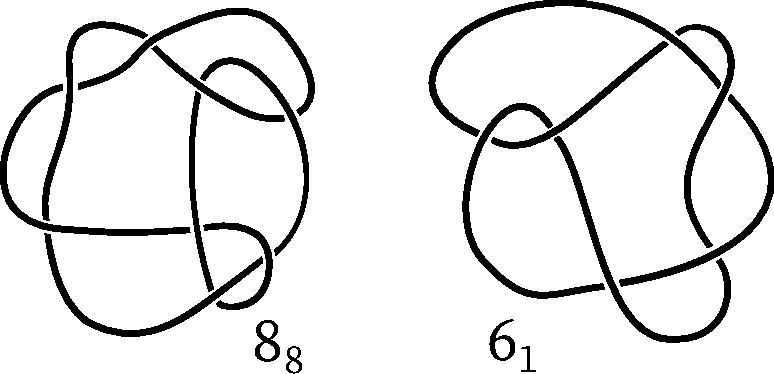
\includegraphics[width=0.45\textwidth]{images/smooth-knots.pdf}
    \caption{Knot diagrams.}%
    \label{fig:diagrams}
\end{figure}

% What is good practice to cite a page number?
Any diagram of a tame (non-wild) knot can be approximated by a regular diagram \cite{murasugi1996}.
Moreover, regular diagrams contain enough information to reconstruct the original knot (up to isotopy). For these reasons it is very convenient to represent knots by regular diagrams, and we will make use of them here frequently.

\subsection{Contact Geometry}

In order to define Legendrian knots we begin by defining a certain plane field on $\R^3$; it is called the \emph{standard contact structure}, or $\xi_0$. At each $(x, y, z) \in \R^3$ we define
\[
    \xi_0(x, y, z) = \lspan \{\partial_y,
                                   \partial_x + y\partial_z\}
\]
Note that $\xi_0$ is defined as a linear combination of the partial derivatives of the coordinate functions, as these are the basis vectors of the tangent space $\tpm_{(x, y, z)} \R^3$, of which $\xi_0$ is a 2-dimensional subspace.

\begin{figure}[ht]
    \centering
    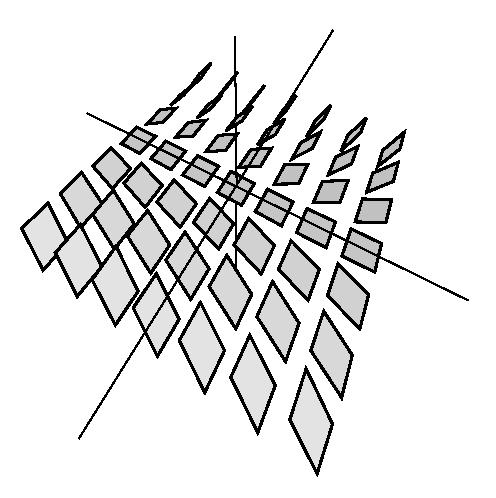
\includegraphics[width=0.5\textwidth]{images/contact-planes.pdf}
    \caption{The standard contact planes in $\R^3$. Diagram from S. Schonenberger.}%
    \label{fig:contact-planes}
\end{figure}
% Add diagram from S. Schonenberger

As we go along the $y$-axis, the plane $\xi_0(p)$  gets steeper and steeper in the $\partial x$ direction. In fact, the planes twist so much that there is no 2-dimensional surface everywhere tangent to $\xi_0$, or even tangent to $\xi_0$ in any open set \cite{boothby}.
% Maybe show the proof with the lie bracket...
Such a plane field is called \emph{completely non-integrable}.
In general, a 3-manifold equipped with a completely non-integrable plane field is called a \emph{contact 3-manifold}.

\textbf{Important!} Every plane field is the kernel of a one-form. In the case of the standard contact planes $\xi_0$, this one form is referred to as $\alpha_0$, and it is given by $\alpha_0 = dz - y \, dx$.

Although no surface can be everywhere tangent to $\xi_0$, there are many curves which run tangent to $\xi_0$. Such a curve is called \emph{Legendrian}, leading to the following definition.

\begin{defn}
    Let $K: (0, 1) \to \R^3$ be a smooth curve. We say $K$ is \textbf{Legendrian} if $K$ is everywhere tangent to $\xi_0$. That is, at all $t \in (0, 1)$,
    \[
        K'(t) \in \xi_0(K(t))
    \]
\end{defn}

As a knot is a smooth embedding of the circle in $\R^3$, so a Legendrian knot is a Legendrian embedding of the circle in $(\R^3, \xi_0)$. But the equivalence relation under which one defines a knot is as important as the curve itself, and so we will define an analogous relation for Legendrian knots. Two knots $K, K'$ are said to be equivalent if there exists a smooth isotopy taking $K$ to $K'$. Similarly, two Legendrian knots $L$ and $L'$ are said to be equivalent if there exists an isotopy taking $L$ to $L'$ such that every intermediate knot is Legendrian.
We frequently use the terms \emph{equivalent} and \emph{isotopic} to refer to knots that are either Legendrian equivalent or smooth equivalent. Generally, when referring to Legendrian knots, we mean Legendrian equivalence, but when confusion may arise we will explicitly use the term \emph{smooth equivalent/isotopic}.

\begin{defn}
    Let $K$ and $K'$ be Legendrian knots. We say $K$ and $K'$ are \textbf{Legendrian equivalent} if there exists a smooth function $\phi: [0, 1] \to \R^3$ such that
    $\phi(0) = K$, $\phi(1) = K'$, and for any $t \in [0, 1]$, $\phi(t)$ is a Legendrian knot.
\end{defn}

By definition, all Legendrian knots are smooth knots, and it is clear that there are representatives of smooth knots which aren't Legendrian. Nonetheless, Legendrian knots are plentiful. In fact, any knot can be $C^0$ approximated by a Legendrian knot (a proof of this fact will be given in section 1.3, once we have defined stabilization).
% TODO: put in this proof 
Such an approximation is smooth isotopic to the target curve, and thus there exist Legendrian representatives of any smooth knot type.

\subsection{Front Diagrams}

Representatives of Legendrian knots are no different from normal knots in that they are curves living in $\R^3$, and so it is convenient to represent them by diagrams.

Unlike smooth knots, Legendrian knots contain geometric information, and so we want our diagrams to record that information too. But because the geometric condition that Legendrian knots satisfy is not invariant under rotation, we must be careful to distinguish which plane we are projecting onto to create a diagram.

There are two projections which are used to represent Legendrian knots. The first is the Lagrangian diagram, which is projection onto the $XY$ plane. This projection is useful in defining certain algebraic invariants, but we will not need it here.
Instead, we restrict our examination to the front projection, which is projection onto the $XZ$ plane such that the positive $Y$ direction points \emph{into} the page.

\begin{figure}[ht]
    \centering
    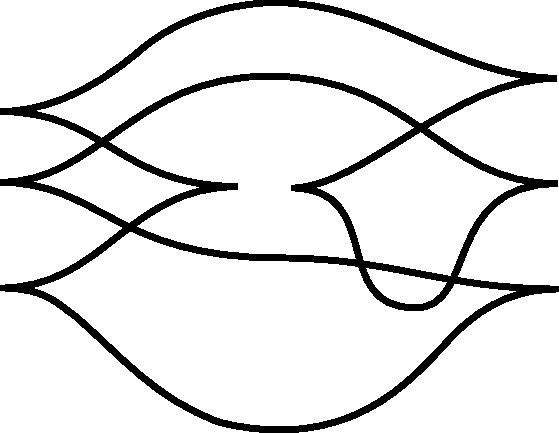
\includegraphics[width=0.3\textwidth]{images/chekanov-1.pdf}
    \hspace{2em}
    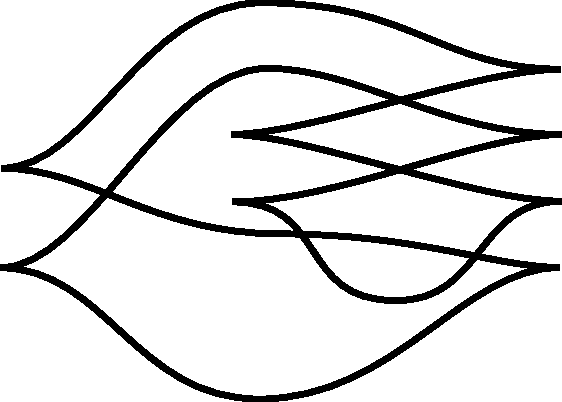
\includegraphics[width=0.3\textwidth]{images/chekanov-2.pdf}
    \caption{Front projections for some Legendrian knots (the Chekanov examples).}%
    \label{fig:front-projection}
\end{figure}

% Could add a proof here..?
Front projections contain enough information to recover the exact geometry of the original knot. This is because the Legendrian condition is a requirement on the tangent based on the $y$-coordinate. Recall that a curve $K$ is Legendrian if $\alpha = dz - y\, dx$ vanishes on $\tpm_p K$ for all $p \in K$. Thus we have $dz - y \, dx = 0$ and thus
\[
    y = \frac{dz}{dx}
\]
This explains the cusps we see on the left and right sides of front diagrams: Since the part above the cusp (which has a negative slope, in the case of a right cusp) and the part below the cusp (which has a positive slope at a right cusp) have to meet, the slopes of each must be zero at the cusp. Note that while these points are cusps in the projection, they are smooth in the 3-dimensional knot.

Moreover, in a front diagram there is no need to mark the overstrand at a crossing: unambiguously, the strand with a more negative slope goes over the other.

\subsection{Classical Invariants}

Any two knots which are Legendrian equivalent are also smooth equivalent by definition, so let us ask whether the converse is true.
As you may expect the answer is no. Moreover, since we can approximate any smooth knot by an isotopic Legendrian one, the relation of Legendrian equivalence ``refines'' the equivalence classes of smooth knots into a larger number of Legendrian equivalence classes. What does the structure of this refinement look like? As expected this is a nontrivial question. We will begin to answer it by looking at equivalence of diagrams.

Although one defines two smooth knots to be equal if there is an isotopy between them as curves in $\R^3$, the Redeimeister moves provide an equivalent \emph{diagrammatic} formulation.
It is three ``moves'' which may be made on a diagram, such that two knots are equal if and only if their diagrams may be related using some series of Redeimeister moves.
The Redeimeister moves don't preserve Legendrian equivalence, but there's a similar set of three diagrammatic moves which determine Legendrian equivalence of front diagrams  \cite{swiatkowski}.

\begin{figure}[ht]
    \centering
    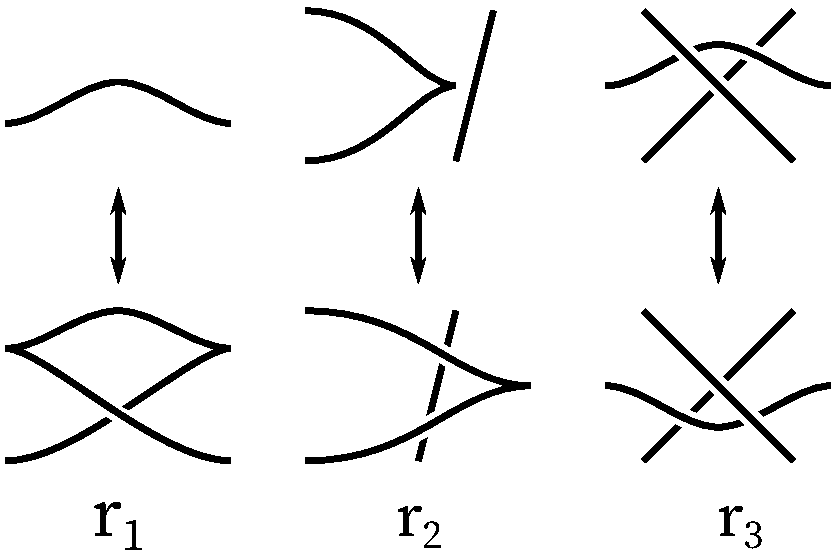
\includegraphics[width=0.5\textwidth]{images/redeimeister.pdf}
    \caption{The Legendrian Redeimeister moves.}%
    \label{fig:redemeister}
\end{figure}

These moves correspond to restricted version of the smooth Redeimeister moves.
Unfortunately, as with the smooth Redeimeister moves, it is difficult in practice to determine equivalence of knots using these rules. Nonetheless, they are useful in the construction of more practical invariants, as invariance under all three Redeimeister moves is equivalent to invariance under Legendrian isotopy.

There are two numerical invariants which can be easily defined in and computed from the front projection, and they are called the \emph{classical invariants}.
\begin{defn}
    Let $K$ be a Legendrian knot, and $D$ a front diagram for $K$. Let $\cusps_r(D)$ be the number of right cusps in $D$, and $\writhe(D)$ the writhe of $D$, defined below.
    Define the \textbf{Thurston-Bennequin number} as
    \[
        \tb(K) = \writhe(D) - \cusps_r(D)
    \]
\end{defn}
To define the writhe $\writhe(D)$ of a diagram $D$, we assign a sign to each crossing in $D$. If as you travel along the overstrand, the understrand goes from right to left, then the crossing is positive; and if the understrand runs from left to right then the crossing is negative. The writhe is the sum of the signs of the crossings.

\begin{figure}[ht]
    \centering
    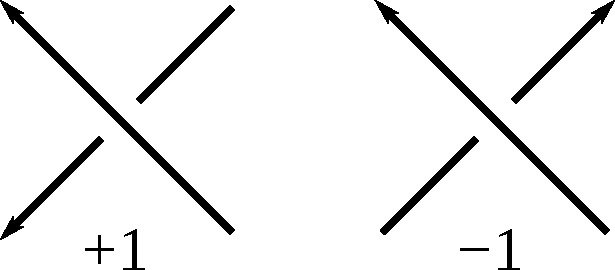
\includegraphics[width=0.3\textwidth]{images/writhe.pdf}
    \caption{The sign at a crossing.}%
    \label{fig:writhe}
\end{figure}

Writhe is \emph{not} an invariant of Legendrian knots. Because the $r_1$ move adds a crossing without changing the orientation of other crossings, it changes the writhe. Nonetheless, the $\tb$ is easily shown to be an invariant.

\begin{proof}
    Let $D$ be a front diagram for a Legendrian knot $K$. It suffices to show that $\tb(D)$ is unchanged under the Legendrian Redeimeister moves.

    \begin{enumerate}
        \item $r_1$ adds one right cusp and one crossing. Regardless of the orientation of of the segment before the move, the new crossing is easily seen to have sign $+1$, and therefore
            \[
                \tb(D') = (\writhe(D) + 1) - (\cusps_r(D) + 1) = \tb(D)
            \]
        \item $r_2$ adds two crossings, but they have opposite signs, so the writhe remains the same.
        \item $r_3$ moves two crossings, but their signs remain unchanged.
    \end{enumerate}
    
\end{proof}

\begin{defn}
    Let $K$ be a Legendrian knot and $D$ a front diagram for $K$. Let $\cusps_u(D)$ be the number of \emph{upward-pointing cusps} and $\cusps_d(D)$ be the number of \emph{downward-pointing cusps}. Define the \textbf{rotation number} of $K$ as 
    \[
        \rot(K) = \frac{1}{2} (\cusps_d(D) - \cusps_u(D))
    \]
    Although $\rot(K)$ is only well-defined for \emph{oriented} $K$, it is defined up to multiplication by $\pm 1$ for unoriented knots.
\end{defn}
\begin{proof}
    As before, we show that $\rot(K)$ is an invariant, so let $D$ be a front diagram for $K$. Neither $r_2$ nor $r_3$ change the orientation or the number of cusps. On the other hand, $r_1$ creates a pair of cusps, one pointing upward and one pointing downward.
\end{proof}

These invariants do a good job of distinguishing Legendrian knots (see \cite{eliashberg2008unknot}), though there are known to be pairs of smooth-isotopic Legendrian knots which have the same TB and rotation number but which are not Legendrian equivalent (\ref{fig:front-projection}, \cite{chekanov}). But the existence of these invariants reveals a great deal about how the Legendrian equivalence classes of a smooth knot are structured. 

\begin{figure}[ht]
    \centering
    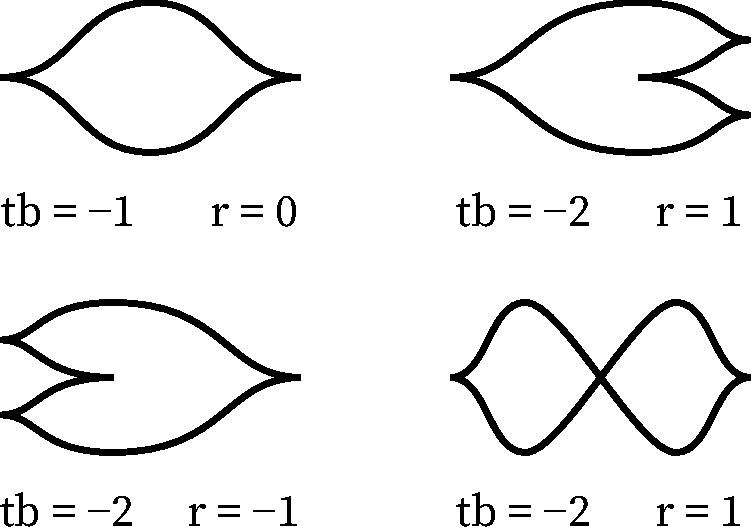
\includegraphics[width=0.4\textwidth]{images/unknots.pdf}
    \caption{A selection of Legendrian unknots.}%
    \label{fig:unknots}
\end{figure}

% Awk
Figure \ref{fig:unknots} shows four Legendrian unknots. One of them has $\tb = -1$ and another has $\tb = -2$, so they aren't isotopic. But the second can be obtained from the first by means of a so-called \emph{stabilization}, shown in figure \ref{fig:stabilization}. 

\begin{figure}[ht]
    \centering
    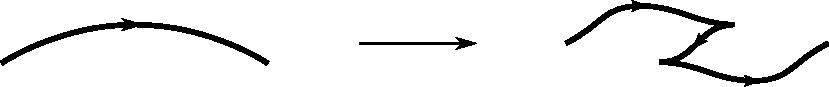
\includegraphics[width=0.6\linewidth]{images/stabilization.pdf}
    \caption{A ``right'' stabilization, increasing the rotation number.}%
    \label{fig:stabilization}
\end{figure}

% Do you need to explicitly mention that stabilization preserves smooth knot type?
A stabilization decreases the TB by 1, and changes the rotation number by $\pm 1$ depending on the orientation. Thus for any smooth knot type, the TBs of its Legendrian representatives are unbounded below, and the rotation numbers are unbounded both above and below.
It is known that for any smooth knot type, the TB is bounded above \cite{bennequin}, and therefore the maximal TB is an invariant of smooth knots. For example, the maximal TB for the unknot is $-1$, as seen in Figure \ref{fig:unknots}. In general, write $\overline{tb}(K)$ for the maximal TB of a smooth knot type.

\subsection{Polynomial Invariants and Skein Relations}

Many useful knot invariants take the form of Laurentian polynomials (ie, having both positive and negative exponents). Typically, these are defined recursively using skein relations, which give an algebraic relationship between the polynomials of knots differing only at a crossing. For certain such relations the resulting knot can be shown to be not only unique, but invariant under isotopy.

In particular, we are interested in the Kauffman polynomial, as it gives an upper bound on the maximal TB of a smooth knot type. We define the Kauffman polynomial in terms of the L-polynomial, which is an invariant only under regular isotopy.
There are many varying definitions of the Kauffman polynomial in the literature. We use here a variant known as the Dubrovnik polynomial (it was discovered in the city of Dubrovnik in Yugoslavia \cite{kauffman}), and we refer to its normalized version as the Kauffman polynomial. Our formulation matches that used by \cite{ferrand} and is similar to that used by \cite{lu-zhong}.

Let $T$ be a link diagram, and define $D$ recursively via the following skein relations, where the Dubrovnik polynomial of the unknot is normalized to be $\frac{a - a^{-1}}{z} + 1$:

\begin{figure}[ht]
    \centering
    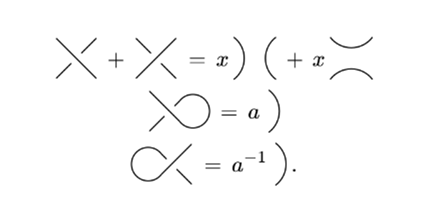
\includegraphics[width=0.5\linewidth]{images/ng-skein.png}
    \caption{The skein relations for the L polynomial, from NG. TODO: make your own diagram, and explain this properly.}%
    \label{fig:skein}
\end{figure}

Yet such a polynomial is certainly not a topological invariant: the $r_1$ move corresponds to multiplication by $a^{\pm 1}$. Thus we normalize the D-polynomial by the writhe to get the Kauffman polynomial $Y(K)$, since the same $r_1$ move which corresponds to a multiplication by $a$ in the Dubrovnik polynomial increases the writhe by 1.
\begin{defn}
    Let $K$ be a smooth knot and $T$ a diagram for $K$. Define the \textbf{Kauffman Polynomial} of $K$ by
    \[
        Y(K) = a^{-w(T)} D(T)
    \]
    The polynomial, which is a Laurentian polynomial in $a, x$, is an invariant under smooth isotopy \cite{kauffman}.
\end{defn}

The degree of the framing variable $a$ in the Kauffman polynomial gives rise to an upper bound on the TB, which was first proved by Rudolph \cite{rudolph}. The version we use here is due to Tabachnikov \cite{tabachnikov}. More information on this bound and its history can be found in \cite{ferrand}.

\begin{theorem}[Kauffman Bound \cite{tabachnikov}]\label{kauffman-bound}
    If $K$ is a Legendrian link, then $\overline{tb}(K) \leq \mu_a(Y(K))$, where $\mu_a(P)$ denotes the minimum degree of $a$ in the polynomial $P(a, x)$.
\end{theorem}

This bound is very useful: there is no method in general for computing the maximal TB of a knot, but it is a fairly straightforward matter to compute its Kauffman polynomial. The bound fails to be sharp in some known cases (eg, \cite{ferrand}) but there are also classes of knots for which it is known to be sharp. These include positive knots, most torus knots, 2-bridge links, and most 3-twist pretzel links. That the Kauffman bound is sharp for many 3-twist pretzel links is a theorem of \cite{ng}:

\begin{theorem}
    Suppose $p_1, p_2, p_3 > 0$. Then the Kauffman bound is sharp for the pretzel links $P(p_1, p_2, p_3)$, $P(-p_1, p_2, p_3)$, and $P(-p_1, -p_2, -p_3)$, and for $P(-p_1, -p_2, p_3)$ when $p_1 \geq p_2 \neq p_3 + 1$.
\end{theorem}

We will make use of this theorem in our main result.

\section{Lagrangian Cobordisms}

\subsection{Symplectic Geometry}

Cobordisms are objects originating in smooth knot theory which define a fundamental relation between types of knots. We define them here in the context of smooth knots, and then we will be able to define a type of cobordism called a Lagrangian cobordism by requiring that it be everywhere tangent to a certain differential form.

\begin{defn}
    Let $K$ and $K'$ be smooth knots. Define a \textbf{cobordism} as a smoothly embedded 2-manifold $A$ in $\R^3 \times I$ such that the bottom edge of $A$ is $K$ and the top edge of $A$ is $K'$. That is,
    \begin{align*}
        A \cap \left(\R^3 \times \{0\}\right) &= K \times \{0\}\\
        A \cap \left(\R^3 \times \{1\}\right) &= K' \times \{1\}
    \end{align*}
\end{defn}

We extend this definition by defining a \emph{symplectic manifold} in much the same way we defined a contact manifold: as a manifold equipped with an appropriate differential form.

\begin{defn}
    Let $X$ be a 4-dimensional smooth manifold and $\omega$ a two-form on $X$ that is closed and nondegenerate. Then the pair $(X, \omega)$ is said to be a \textbf{symplectic 4-manifold}.
\end{defn}

Analogous to Legendrian curves in contact manifolds are Lagrangian surfaces in symplectic manifolds.
\begin{defn}
    Let $(X, \omega)$ be a symplectic 4-manifold and $L$ a smoothly embedded 2-manifold in $X$. We say $L$ is \textbf{Lagrangian} if for all $p \in L$, $\omega$ vanishes on $\tpm_p L$.
\end{defn}

% This section could do with a rework -- either go more into depth or less into depth.

% give a citation for this
Given a contact manifold $(Y, \ker \alpha)$ there is a canonically associated symplectic manifold $(Y \times \R, d(e^t \alpha))$, where $t$ is the coordinate on the attached copy of $\R$. This allows us to put Legendrian knots into symplectic manifolds as slices of Lagrangian submanifolds. Thus a Lagrangian cobordism is a cobordism that is also Lagrangian, with a few extra conditions required.

\begin{defn}
    Let $K$, and $K'$ be Legendrian links, and $L$ a Lagrangian manifold in $(\R^3 \times \R, d(e^t \alpha))$. We say $L$ is a \textbf{Lagrangian cobordism} between $K$ and $K'$ if for some $T > 0$,
    \begin{align*}
        L \cap \left(\R^3 \times (-\infty, -T)\right) &= K \times (-\infty, -T)\\
        L \cap \left(\R^3 \times (T, \infty)\right) &= K' \times (T, \infty)\\
        L \cap \left(\R^3 \times [-T, T] \right)\, &\,\, \text{is compact}
    \end{align*}
    and there exists a function $f: L \to \R$ such that $df = e^t \alpha |_{\tpm L}$ and $f$ is constant above $t = T$ and below $t = -T$.

    We call a Lagrangian cobordism between two \emph{knots} (excluding links with multiple components) with genus zero a \emph{concordance.}
\end{defn}

\begin{figure}[ht]
    \centering
    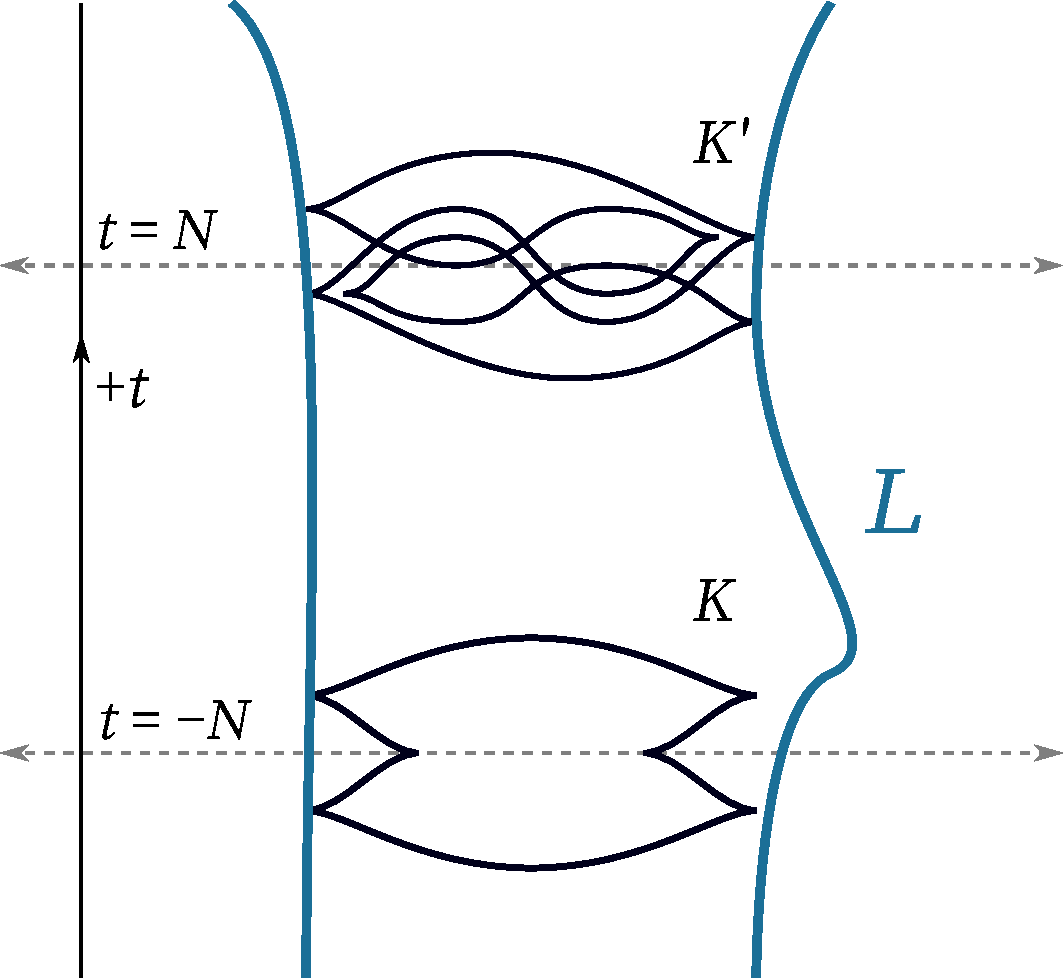
\includegraphics[width=0.4\textwidth]{images/cobordism-visualization.pdf}
    \caption{A visualization of a Lagrangian cobordism $L$ as a cylinder with two Legendrian knots at the ends. Each slice along the $t$ axis is an entire $\R^3$. In this diagram $K$ is the unknot and $K'$ is $m(6_1)$.}%
    \label{fig:cobordism-vis}
\end{figure}

% be more precise here
The change in definition from looking at intersections of the cobordism with $\R^3$-planes to looking at intersections with entire rectangular regions is due to the differential structure of the symplectic manifold; it does not change the nature of the relation. What is more important is that we have added an asymmetric geometric condition on the cobordism, and the result is that the relation "there exists a Lagrangian cobordism from $K$ to $K'$" is not symmetric.

We make the distinction between cobordisms with genus and concordances because the genus of a cobordism gives a lot of information about the two knots at its ends \cite{chantraine2010}. In particular, if $L$ is a cobordism between $K$ and $K'$, then
\[
    \rot(K) = \rot(K') \text{     and     } \tb(K) - \tb(K') = \chi(L)
\]
Thus a Lagrangian concordance can only exist between two knots with equal rotation number and TB.


\subsection{Constructable Cobordisms}

In general, Lagrangian cobordisms are difficult to find. However, there are several conditions in which they are known to exist. Of interest is a certain set of moves which may be easily defined on front diagrams, the Redeimeister moves among them, such that a Langrangian cobordism exists between knots related by them.

\begin{theorem}[\cite{bourgeois15}]
    Suppose $K$ and $K'$ are Legendrian knots. If the front diagram of $K'$ can be obtained from the front diagram of $K$ by a finite sequence of handle moves (figure \ref{fig:handles}) and Redeimeister moves (figure \ref{fig:redemeister}), then there exists a Lagrangian cobordism from $K$ to $K'$. 
\end{theorem}
\begin{figure}[ht!]
    \centering
    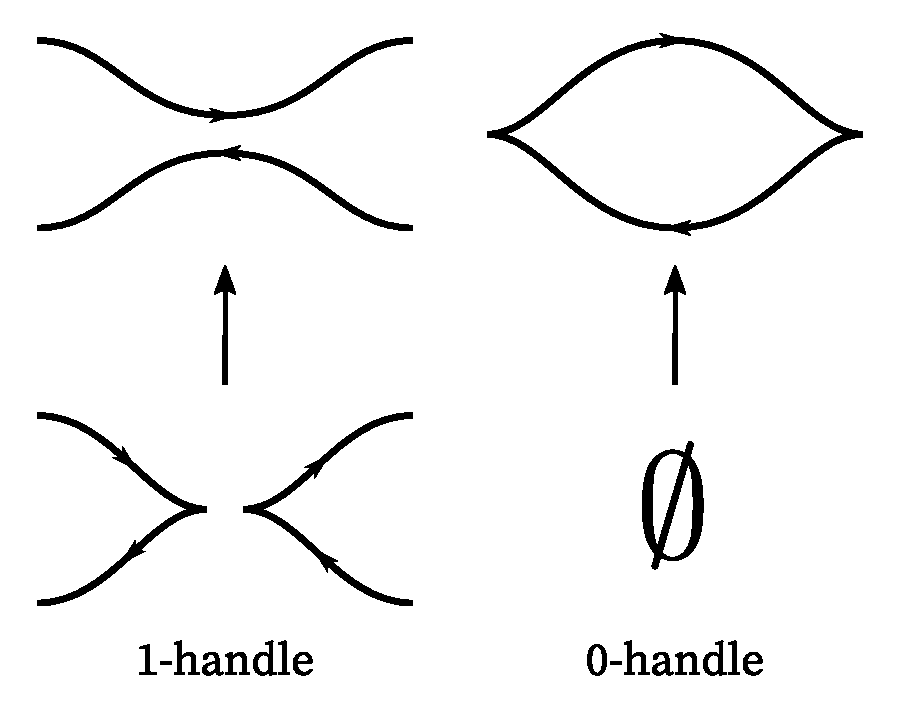
\includegraphics[width=0.4\textwidth]{images/handles.pdf}
    \caption{The handle moves. Note that these moves are one-directional, unlike the Redeimeister moves. The addition of a one-handle is sometimes referred to as a \emph{pinch move}. The addition of a zero-handle corresponds to adding an unlinked unknot with maximal TB to the diagram.}
    \label{fig:handles}
\end{figure}

We refer to a cobordism that is a result of a sequence of these moves as \textbf{constructible}. We can represent these cobordisms visually via a sequence of front diagrams of Legendrian links, each of which is obtained from the previous by one of the constructible moves. For example, figure \ref{fig:cobordism-construction} shows a movie for a constructible cobordism from a double-stabilized unknot to a Legendrian representative of $m(6_1)$.

\begin{figure}[ht!]
    \centering
    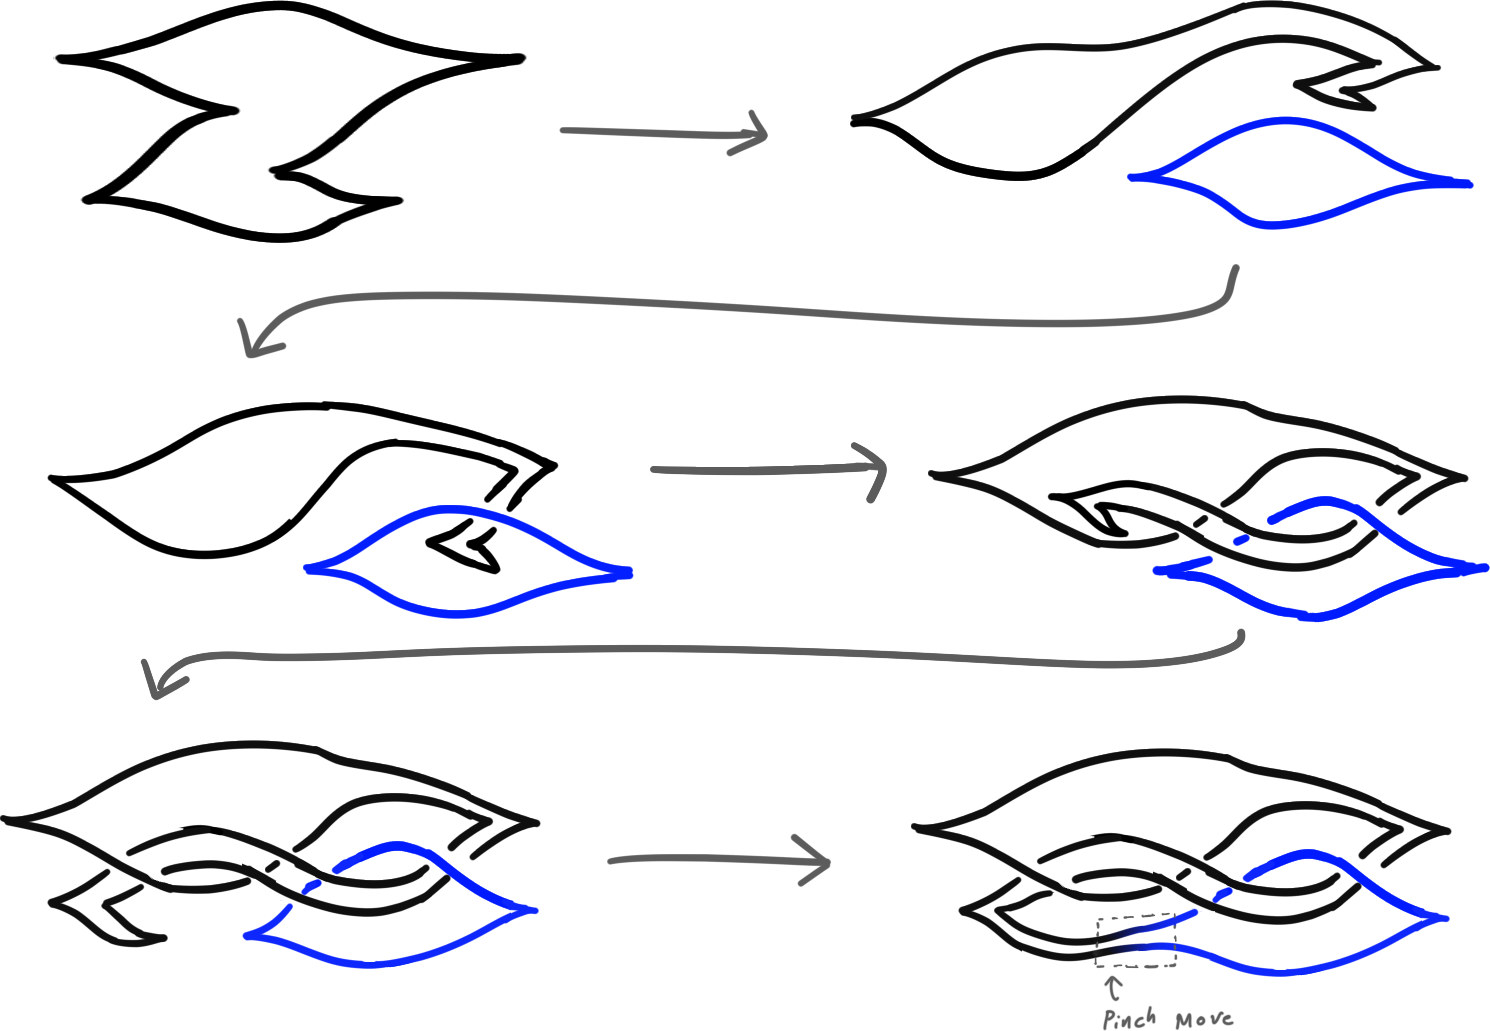
\includegraphics[width=0.5\textwidth]{images/cobordism-construction.png}
    \caption{Constructing a cobordism from the unknot to $m(6_1)$.
    TODO: Make a real nice SVG diagram for this.}%
    \label{fig:cobordism-construction}
\end{figure}

It is known that not all Lagrangian cobordisms are constructible. Moreover, there exist pairs of knots $K, K'$ such that a Lagrangian cobordism exists from $K$ to $K'$ but no such constructible cobordism exists. Specifically, there exists a Lagrangian cobordism from the unknot to the empty set, despite the fact that no constructible move can give $\emptyset$ from a nonempty Legendrian. It is not known whether this is the case when $K' \neq \emptyset$.

\section{Ribbon, Pretzel, etc}

Finding Langrangian cobordisms is hard, and it's not much easier to even know when they exist.
A natural way of refining this question is to restrict one of the knots.
Specifically, we want to know under what conditions there exists a constructible cobordism from the unknot $U$ to some Legendrian knot $K$. TODO: Explain more about this question.

A good candidate for this search is the class of knots called ribbon knots, which we define here.

\begin{defn}
    A knot $K$ is said to be \textbf{ribbon} if $K$ bounds a smoothly embedded disk $d: D \to \R^3$ with only ribbon singularities.
    That is, every region of self-intersection of $d$ is an arc $A \in \R^3$ such that the preimage of $A$, $d^{-1} (A)$, consists of two arks in $D$ of which one is within the interior of $D$ and the other has its endpoints on the boundary of $D$.
\end{defn}

This definition is more clear alongside a ribbon diagram.

\begin{figure}[ht!]
    \centering
    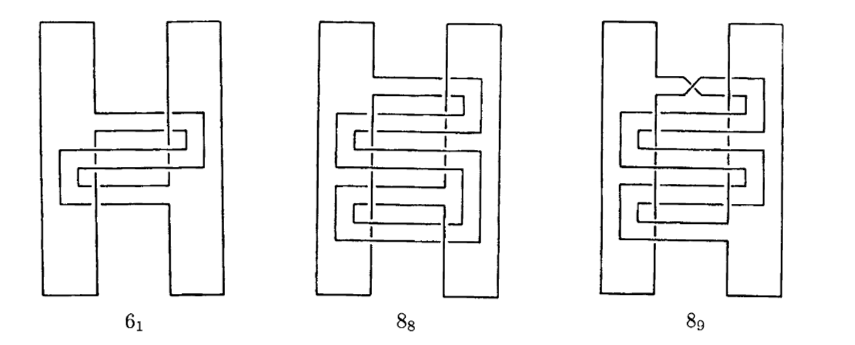
\includegraphics[width=0.8\linewidth]{images/ribbon-knots-kawauchi.png}
    \caption{Ribbon Diagrams, from Kawauchi. TODO: Make your own}%
    \label{fig:ribbon-knots-kawauchi}
\end{figure}

In the smooth world, there are fundamental connections between ribbon knots and cobordisms \cite{fox-milnor}. TODO: Explain this

Similarly, for Legendrian knots it is clear that ribbon knots can be constructed from a sufficiently stabilized unknot using the Redeimeister moves, one 0-handle, and one 1-handle. 
Starting from the unknot, we add a second unknot with a zero-handle, and then use Legendrian isotopy to "pass" the tip of the first unknot through the two loops as desired, before finally using a 1-handle to join the ribbon tip to the second unknot, thus closing the knot. 
TODO: give a better "proof".

The cobordism created by these moves is necessarily a concordance: The surfaces corresponding to each unknot have genus zero before the addition of the 1-handle, which connects them in only one place.
TODO: is this explanation right?

Thus to construct such a cobordism to a ribbon knot $K$, we have to start with an unknot $U$ with $\tb U = \tb K$. Given the topological knot type of $K$, the unknot and $K$ must certainly have $\tb \leq \overline{\tb} K$.
It is an open question when this can be achieved with equality: that is, when a cobordism can be constructed from a stabilized unknot to a maximal-TB Legendrian ribbon knot. 

The main result of this project is the demonstration of a family of ribbon knots for which such a cobordism may be constructed with maximal Thurston-Bennequin number.



\appendix

\printbibliography
\end{document}
